%Dokumentklasse
\documentclass[a4paper, ngerman, 12pt]{scrreprt}

%Seitenränder
\usepackage[top = 2.5 cm, left= 3.5cm, right = 2.5cm, bottom = 3 cm]{geometry}

%Zeilenabstand
%\usepackage[onehalfspacing]{setspace}

% ==== Packages ====

%Dokumentinformationen
\usepackage[
	pdftitle={},
	pdfsubject={},
	pdfauthor={Thomas Zenger},
	pdfkeywords={},	
	%Rahmen von Links verbergen
	hidelinks
]{hyperref}


%Standard Packages
\usepackage[utf8]{inputenc}
\usepackage[T1]{fontenc}
\usepackage{lmodern}

\usepackage{babel}
\usepackage{color, colortbl}
\usepackage{graphicx, subfig}
\usepackage{float}

\usepackage{textcomp}
\usepackage{listings}

\usepackage{amssymb} 
\usepackage{mathtools}

\usepackage{fancyhdr}

%nicht einrücken nach Absatz
\setlength{\parindent}{0pt}

%Farben
\definecolor{lstback}{RGB}{240, 240, 240}
\definecolor{darkgreen}{RGB}{0, 100, 0}
\definecolor{dgreen}{RGB}{219, 169, 1}
\definecolor{Gray}{gray}{0.9}

%Codelisings - Sprache angeben
\lstset{
	language=c,
	numbers=left,
	stepnumber=1,
	frame=single,
	captionpos=b,
	backgroundcolor=\color{lstback},
	breaklines=true,
	commentstyle=\color{green},
	keywordstyle=\color{blue} \textbf,
	identifierstyle=\color{black},
	stringstyle=\color{darkgreen}\ttfamily,
	basicstyle = \ttfamily \color{black} \footnotesize,
	inputencoding=utf8,
	showstringspaces=false,
	escapeinside={@}{@}
}

%Trennung
%\hyphenation()

%Redefine
\renewcommand{\headrulewidth}{0.4pt}
\renewcommand{\footrulewidth}{0.4pt}

% ==== Kopf- und Fußzeile ====
\pagestyle{fancy}
\fancyhf{}
\lhead{}
\chead{}
\rhead{\leftmark}
%%
\lfoot{Thomas Zenger}
\cfoot{}
\rfoot{\thepage}
%%



\begin{document}

%Titelseite
\begin{titlepage}
\begin{center}
\vspace*{3cm}
\huge\textbf{\texttt{B1B}}\\
\vspace{1cm}
{\fontsize{50}{48} \selectfont Back in Business}\\
\vspace{0.5em}
%Thematik
{\fontsize{40}{48} \selectfont Git}\\
\end{center}
\vspace{\fill}
%Author
\begin{large}
Thomas Zenger\\
mail@thomas-zenger.de\\
20.08.2017\\
\end{large}
\vspace{2cm}
\end{titlepage}


\pagestyle{fancy}
%Inhaltsverzeichnis
\tableofcontents
%Verzeichnis aller Bilder
\listoffigures
%Verzeichnis aller Tabellen
\listoftables
%Verzeichnis aller Code Listings
\lstlistoflistings


%Teildokumente einfügen
\pagestyle{fancy}
\chapter{Vorwort}
\section{\texttt{B1B} - Was ist das?}
Dieses Skript soll als Nachschlagewerk und Cheat Sheet dienen und eine Gedächtnisstütze zu einem bereits vertiefeten Thema bieten. Es soll keine Fachliteratur ersetzen und dient auch nicht zum Erlernen der Thematik, da auf ausführliche Erklärungen größtenteils verzichtet wird.
\section{Motivation}
Diese Idee zu diesem Kompendium enstand während meines Informatikstudiums. Da bereits erlernte Techniken, wie z.B. Programmier- oder Scriptsprachen, mit dem Fortschreiten des Studiums in den Hintergrund traten, zu einem späteren Zeitpunkt jedoch wieder benötigt wurden, war es unerlässlich sich diese wieder ins Gedächtnis zu rufen. Aus diesem Grund entstand dieses Werk als eine Art ``erweiterte Zusammenfassung''.
\section{Literatur und Grundlagen}
Folgende Werke fanden bei der Erstellung dieses Dokuments Beachtung. An dieser Stelle soll ausdrücklich erwähnt werden, dass sich diese Arbeit nicht als Plagiat oder Kopie genannter Literatur verstanden werden soll, sondern als Lernhilfe und Zusammenfassung.
\begin{itemize}
\item Git Documentation https://git-scm.com/doc
\end{itemize}

\chapter{Einführung}
\section{Versionskontrolle}
Versionskontrollsysteme protokollieren Änderungen an Dateinen und ermöglichen es zu jedem Zeitpunkt auf eine ältere Version zuzugreifen.
\section{Git}
Im Gegensatz zu zentralen Versionskontrollsystemen handelt es sich bei Git um ein verteiltes Versionskontrollsystem (DVCS). Jeder Anwender clont das komplette Repository und erhält somit eine vollständige Kopie des Projektes.
\begin{figure}[ht]
	\centering
		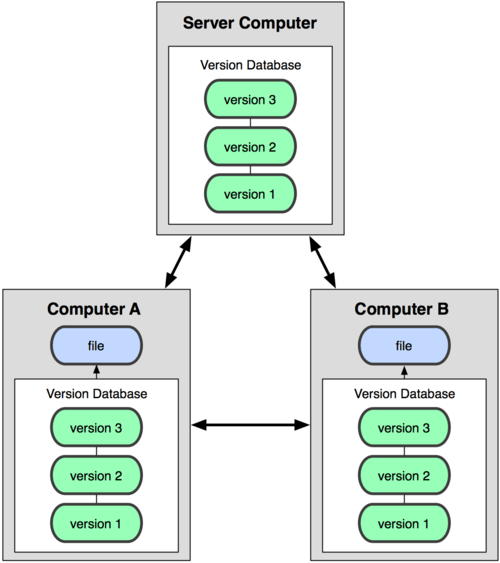
\includegraphics[width=0.5\textwidth]{img/dvcs.png}
	\caption{Verteilte Versionskontrolle}
\end{figure}
\subsection{Arbeitsweise}
Git speichert bei jedem Commit nur die geänderten Dateien. Nicht geänderte Dateien werden mit einem Verweis auf die alte Version übernommen. Es werden keine Informationen von anderen Rechnern im Netzwerk benötigt, da Git fast alle Operationen lokal ausführt und die Informationen ebenfalls in einer lokalen Datenbank hinterlegt werden. Änderungen werden zur Sicherstellung der Integrität mit Check\-summen überprüft.
\begin{figure}[ht]
	\centering
		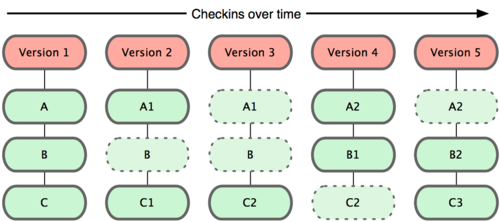
\includegraphics[width=0.6\textwidth]{img/snap.png}
	\caption{Git Snapshots}
\end{figure}
\subsection{3 Zustände}
Git definiert drei Hauptzustände, in denen sich eine Datei befinden kann. 
\begin{itemize}
\item \textbf{commited}\\
Daten sind in der lokalen Datenbank gesichert
\item \textbf{modified}\\
Datei wurde geändert, aber noch nicht commited
\item \textbf{staged}\\
Datei im gegenwärtigen Zustand für nächsten Commit vorgemerkt
\end{itemize}
\section{Git Config}
Git kann per Config Dateien angepasst werden. Der Befehl \texttt{git config} führt alle Optionen auf.
\section{Manpage}
Die Manpage hat den Vorteil, dass sie auch offline aufgerufen werden kann. Folgende Befehle stehen zur Auswahl:
\begin{lstlisting}[caption={Git Manpage},captionpos=b]
git help <verb>
git <verb> --help
man git-<verb>
\end{lstlisting}

\chapter{Grundlagen}
\section{Git Repository anlegen}
\subsection{Existierendes Verzeichnis initialisieren}
Ein bereits existierendes Verzeichnis kann als Git Repository initialisiert werden. Dabei wird ein Unterverzeichnis \texttt{.git} angelegt. Bereits im Verzeichnis erhaltene Daten werden nicht automatisch versioniert. Dies geschieht mit dem ersten Commit.\\
\begin{lstlisting}[caption={Initialisierung},captionpos=b]
git init
\end{lstlisting}
\subsection{Existierendes Repository klonen}
Um eine Kopie eines existierenden Projekts zu erstellen wird dieses geklont. Alle bereits vorhandenen Daten werden als lokale Kopie des Projekts gespeichert. Dabei wird ein Verzeichnis mit dem Namen des Projekts angelegt.\\
\begin{lstlisting}[caption={Clone},captionpos=b]
git clone [url]

#Eigener Verzeichnisname
git clone [url] newDir
\end{lstlisting}
\section{Änderungen nachverfolgen}
Dateien im Arbeitsverzeichnis können entweder verfolgt (tracked) oder nicht verfolgt (untracked) werden. Alle Dateien des letzten Commits befinden sich in der Versionskontrolle. Diese Dateien können unverändert (unmodified), verändert (modified) oder für den nächsten Commit vorgemerkt (staged) vorliegen. Alle anderen Dateien sind nicht versioniert (Nicht im letzten Commit und nicht in der Staging Area).
\begin{figure}[H]
	\centering
		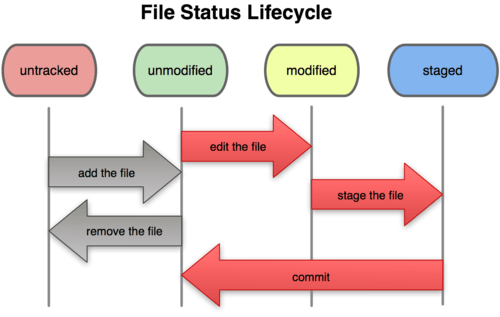
\includegraphics[width=0.6\textwidth]{img/follow.png}
	\caption{File Status LC}
\end{figure}
\section{Status prüfen}
\begin{lstlisting}[caption={Status},captionpos=b]
git status
\end{lstlisting}
\section{Dateien hinzufügen}
\begin{lstlisting}[caption={Add},captionpos=b]
git add newFile
\end{lstlisting}
\section{Dateien stagen}
\begin{lstlisting}[caption={Stage},captionpos=b]
git add existingFile
\end{lstlisting}
\section{Dateien ignorieren}
In der Datei \texttt{.gitignore} können Regeln hinterlegt werden, welche Dateien von Git ignoriert werden sollen.
\section{Staging Area durchsuchen}
Um die Staging Area und das Arbeitsverzeichnis direkt zu vergleichen kann \texttt{diff} benutzt werden.
\begin{lstlisting}[caption={Diff},captionpos=b]
git diff
\end{lstlisting}
\section{Commit aus Staging Area erzeugen}
\begin{lstlisting}[caption={Commit},captionpos=b]
#Editor
git commit

#Editor mit diff
git commit -v

#Meldung direkt angeben
git commit -m ''Message from Hell''
\end{lstlisting}
\section{Staging Area überspringen}
Alle Dateien, welche sich bereits unter Versionskontrolle befinden, werden im Commit aufgenommen.
\begin{lstlisting}[caption={Commit w/o Staging Area},captionpos=b]
git commit -a
\end{lstlisting}
\section{Dateien entfernen}
\subsection{Staging Area}
\begin{lstlisting}[caption={RM Staging Area},captionpos=b]
git rm --cached file.txt
\end{lstlisting}
\subsection{Arbeitsverzeichnis}
\begin{lstlisting}[caption={RM},captionpos=b]
#delete file
rm file.txt
#staging area
git rm file.txt
#commit
git commit
\end{lstlisting}
\section{Dateien verschieben}
Git verfolgt nicht explizit, ob Dateien verschoben werden.
\begin{lstlisting}[caption={Move},captionpos=b]
git move file_from file_to
\end{lstlisting}
\section{Historie}
Der Befehl \texttt{git log} listet alle Commits eines Projekts in umgekehrter chronologischer Reihenfolge auf. Mit Hilfe von Optionen kann bestimmt werden, welche Informationen angezeigt werden sollen.\\
\begin{lstlisting}[caption={Log},captionpos=b]
#normal
git log

#display changes (diff)
git log -p

#diff by words not lines
git log -p --word-diff

#statistc
git log --stat

#one commit per line
git log --pretty=online

#branch graph
git log --pretty=oneline --graph
\end{lstlisting}
\begin{center}
\renewcommand{\arraystretch}{1.2}
\begin{tabular}{|p{4cm}p{10cm}|}
\hline
\textbf{Option}				&\textbf{Beschreibung}\\
\hline
\texttt{-p}					&Zeigt Patch eines Commits\\
\hline
\texttt{-{}-word-diff}			&Vergleich Wort zu Wort\\
\hline
\texttt{-{}-stat}				&Statistik der geänderten Dateien und entfernten/hinzugefügten Zeilen\\
\hline
\texttt{-{}-startstat}			&Kurzstatistik über eingefügte/entfernte Zeilen\\
\hline
\texttt{-{}-name-only}			&Liste der geänderten Dateienen nach Commit Informationen\\
\hline
\texttt{-{}-name-status}		&Liste der Dateien mit hinzufügt/geändert/entfernt Statistik\\
\hline
\texttt{-{}-abbrev-commit}		&Zeigt nur erste Zeichen einer SHA-1 Checksum\\
\hline
\texttt{-{}-relative-date}		&Zeigt Datum in relativen Format\\
\hline
\texttt{-{}-graph}				&ASCII Graph der Branch- und Merch-Historie\\
\hline
\texttt{-{}-pretty}				&Zeigt Commits in alternativen Format (online, short, full, fuller und format [eigenes Format spezifizieren])\\
\hline
\end{tabular}
\captionof{table}{Log Options Format}
\renewcommand{\arraystretch}{1}
\end{center}
\newpage
\subsection{Log Dateien Filtern}
Außerdem stehen weitere Optionen zur Verfügung, die zur Filterung der Ergebnisse dienen.
\begin{center}
\renewcommand{\arraystretch}{1.2}
\begin{tabular}{|p{4cm}p{10cm}|}
\hline
\textbf{Option}				&\textbf{Beschreibung}\\
\hline
\texttt{-(n)}					&Ausgabe von n Commits\\
\hline
\texttt{-{}-since, -{}-after}		&Commits nach dem angegebenen Datum\\
\hline
\texttt{-{}until, -{}-before}		&Commits vor dem angegebenen Datum\\
\hline
\texttt{-{}-author}			&Commits von angegebenen Author\\
\hline
\texttt{-{}-committer}			&Commits vcon angegebenen Committer\\
\hline
\texttt{-{}-no-merges}			&Commits welche keine Merges sind\\
\hline
\end{tabular}
\captionof{table}{Log Options Format}
\renewcommand{\arraystretch}{1}
\end{center}
\section{Änderungen rückgängig machen}
\subsection{letzten Commit ändern}
Ändert den letzten Commit (vergessene Dateien hinzufügen, Message ändern). Direkt nach dem letzten Commit auszuführen, wenn noch keine weiteren Änderungen gemacht wurden (Staging Area wird verwendet).\\
\begin{lstlisting}[caption={letzten Commit ändern},captionpos=b]
#texteditor new message
git commit --amend

#add forgotten file
git commit -m 'initial commit'
git add forgotten_file
git commit --amend
\end{lstlisting}
\subsection{Änderungen aus Staging Area entfernen}
\begin{lstlisting}[caption={Entfernen aus Staging Area},captionpos=b]
#list files in staging area
git status

#remove file from staging area
git reset HEAD <file>
\end{lstlisting}
\subsection{Änderungen an einer Datei rückgängig machen}
\begin{lstlisting}[caption={Änderungen an Datei rückgängig machen},captionpos=b]
#file status last commit
git checkout -- <file>
\end{lstlisting}
\section{Externe Repositorys}
\subsection{Remote Repositorys anzeigen}
\begin{lstlisting}[caption={Repo anzeigen},captionpos=b]
#display remote server
git remote

#display remote server with url
git remote -v
\end{lstlisting}
\subsection{Remote Repository hinzufügen}
\begin{lstlisting}[caption={Repo hinzufügen},captionpos=b]
#add repo with shortname
git remote add [shortname] [url]
\end{lstlisting}
\subsection{Änderunges aus Remote Repository herunterladen und zusammenführen}
\begin{lstlisting}[caption={Repo zusammenführen},captionpos=b]
#download changes without merging
git fetch [remote-name]

#download changes with merging (only if branch tracked)
git pull
\end{lstlisting}
\subsection{Änderunges hochladen}
\begin{lstlisting}[caption={Änderungen hochladen},captionpos=b]
#upload changes
git push [remote-name] [branch-name]
\end{lstlisting}
\subsection{Repository ansehen}
\begin{lstlisting}[caption={Repository ansehen},captionpos=b]
#display remote repository
git remote show [remote-name]
\end{lstlisting}
\subsection{Verweise auf Remote Repository}
\begin{lstlisting}[caption={Verweise auf Remote Repo},captionpos=b]
#rename
git remote rename name newName

#remove
git remote rm name
\end{lstlisting}
\section{Tags}
\subsection{Tags anzeigen}
\begin{lstlisting}[caption={Tags anzeigen},captionpos=b]
#display tags alphabetical
git tag

#display only versions that belong to 1.x
git tag -l 'v.1.*'
\end{lstlisting}
\subsection{Tags anlegen}
Git bietet zwei verschiedene Typen von Tags an. einfache Tags (lightweight) und kommentierte (annotated) Tags. Ein einfacher Branch ist ein Zeiger auf einen bestimmten Commit. Kommentierte Tags werden als Objekte in Git gespeichert.\\
\begin{lstlisting}[caption={Tags anlegen (Teil 1)},captionpos=b]
#lightweight tag
git tag v1.0

#annotated tag
git tag -a v1.0

#annotated tag with message
git tag -a v1.0 -m 'first release version'

#annotated GPG signed tag with message
git tag -s v1.0 -m 'first release version'

#verify signed tag
git tag -v [tagname]

#display tag
git show [tagname]
\end{lstlisting}
\newpage
\begin{lstlisting}[caption={Tags anlegen (Teil 2)},captionpos=b]
#tag afterwards
git tag -a [tagname] -m [message] [hash]

#upload tag
git push origin [tagname]

#upload all tags
git push origin --tags
\end{lstlisting}
\section{Auto-Vervollständigung}
Mit Hilfe eines Bash Scriptes ist es möglich eine Auto-Vervollständigung für die Bash auf Linux Systemen einzurichten. Das Script kann von folgender Quelle bezogen werden: \\
\texttt{https://github.com/git/git/blob/master/contrib/completion/git-completion.bash }
Im Verzeichnis \texttt{/etc/bash\_completion.d/} ist nun eine Datei mit dem Namen\newline
\texttt{git-completion.bash} anzulegen. Mit \texttt{Tab} kann nun die Autovervollständigung erfolgen (2 mal drücken für Vorschläge).
\section{Git Aliase}
In Git können Aliase dazu verwendet werden um häufig verwendete Befehle abzukürzen.\\
\begin{lstlisting}[caption={Alias},captionpos=b]
git config --global alias.[name] [befehl]
\end{lstlisting}
\chapter{Branching}
\section{Begriffserklärung}
Bei einem Commit speichert Git ein Commit-Objekt ab. Dieses Objekt enthält einen Zeiger auf den Snapshot mit den Objekten der Staging Area, Autor, Metadaten und einen Zeiger auf die direkten Eltern-Commits. Projektverzeichnisse werden als tree-Objekt abgelegt und Projektdateien als Blob gespeichert.
\begin{figure}[htb]
    \centering
    \begin{minipage}[t]{0.48\linewidth}
        \centering
        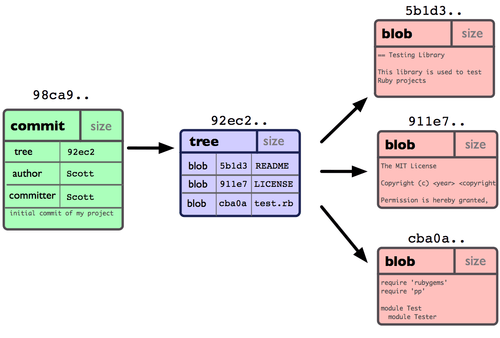
\includegraphics[width=\linewidth]{img/tree.png}
        \caption{Commit Daten}
    \end{minipage}% <- sonst wird hier ein Leerzeichen eingefügt
    \hfill
    \begin{minipage}[t]{0.48\linewidth}
        \centering
        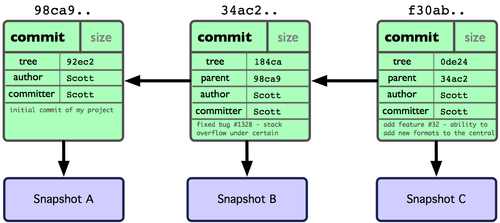
\includegraphics[width=\linewidth]{img/commits.png}
        \caption{mehrere Commits}
    \end{minipage}
\end{figure}
Ein Branch in Git ist ein Zeiger auf einen dieser Commits. Der Standard Git Branch heißt \texttt{master}. Dieser wird mit dem Initial Commit erstellt. Beim Erstellen eines neuen Branches wird ein neuer Zeiger erstellt. Dieser zeigt auf den gleichen Commit, auf welchem gerade gearbeitet wird. Dies wird über den HEAD-Zeiger realisisert, welcher auf den aktullen lokalen Branch zeigt.
\begin{figure}[ht]
	\centering
		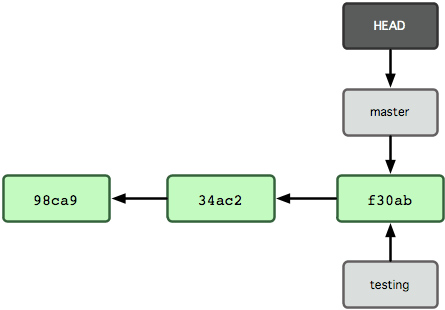
\includegraphics[width=0.6\textwidth]{img/branch.png}
	\caption{Branch erstellen}
\end{figure}
\newpage
\section{Branch anlegen}
\begin{lstlisting}[caption={Branch anlegen},captionpos=b]
#create branch
git branch [branchname]

#create branch, activate and switch to it
git checkout -b [branchname]
\end{lstlisting}
\section{Branch wechseln}
\begin{lstlisting}[caption={Branch wechseln},captionpos=b]
git checkout [branchname]
\end{lstlisting}
\section{Arbeiten mit Branches}
Auf jeden Branch kann unabhängig zu anderen Branches gearbeitet werden. Beim Wechseln des Branches wird lediglich der HEAD Zeiger verschoben und alle Dateien im Arbeitsverzeichnis auf den Stand des letzten Commits des Branches in den gewechselt wird versetzt. Commitete Änderungen des anderen Branches bleiben natürlich erhalten. Da Branches selbst keinerlei Dateien enthalten und nur aus einer kleinen Datei bestehen (SHA-1 Prüfsumme), können diese einfach erstellt und entfernt werden.
\begin{figure}[ht]
	\centering
		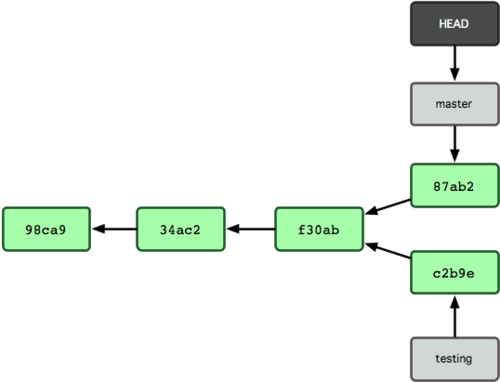
\includegraphics[width=0.8\textwidth]{img/branches.png}
	\caption{Verzweigte Branches}
\end{figure}
\newpage
\section{Einfaches Branching und Merging}
Änderungen, Verbesserung, etc. sollten nicht im Produktivzweig erstellt werden. Hierzu ist es ratsam einen extra Branch für die Entwicklung zu erstellen. Hierzu ein einfaches Beispiel anhand einer Webentwicklung:
\begin{lstlisting}[caption={Einfaches Merging Beispiel},captionpos=b]
#Branch erstellen
git branch dev

#Branch wechseln
git checkout dev

#Entwicklung
vim index.html

#Commit
git commit -a -m 'Content added'

#Zum Master Branch wechseln und zusammenfuehren von Master und Dev
git checkout master
git merge dev

#Entwicklungsbranch entfernen
git branch -d dev
\end{lstlisting}
\section{Grundlagen des Zusammenführens (Merge)}
\begin{center}
\renewcommand{\arraystretch}{1.2}
\begin{tabular}{|p{4cm}p{10cm}|}
\hline
\textbf{Vorgehen}			&\textbf{Beschreibung}\\
\hline
\texttt{fast forward}			&Neuer Commit direkter Nachfolger von ursprünglichen Commit. Einfaches Merging. Zeiger wird einfach auf neuen Commit weiter bewegt (kein neuer Commit).\\
\hline
\texttt{recursive strategy}		&Kein direkter Nachfolger. 3-Wege-Merge. Neuer Commit wird angelegt. Git ermittelt selbstständig die besten 3 Eltern (merge commit).\\
\hline
\end{tabular}
\captionof{table}{Merge Strategien}
\renewcommand{\arraystretch}{1}
\end{center}
\section{Merge Konflikte}
Wurden an den selben Stellen in den selben Dateien unterschiedlicher Branches etwas geändert, können diese Änderungen von Git nicht sauber zusammengefügt werden. Dies führt zu einen Merge Conflict. Diese Dateien werden als \texttt{unmerged} aufgelistet und mit Markern versehen um die Konflikte manuell zu lösen. Nach dem Auflösen des Konflikts müssen die Dateien per \texttt{git add} der Staging Area hinzugefügt werden. Das Staging markiert sie für Git als gereinigt. Anschließend nochmals mit \texttt{git status} überprüfen, ob alle Konflikte aufgelöst wurden und den Merge mit \texttt{git commit} abschießen.
\section{Branch Management}
\begin{lstlisting}[caption={Branch Management},captionpos=b]
# list branches
git branch

#last commit per branch
git branch -v

#display only merged branches
git branch --merged

#display only unmerged branches
git branch --unmerged

#branches with unmerged changes
git branch --no-merged

#delete branch with unmerged changes
git branch -D [branchname]
\end{lstlisting}
\section{Workflows}
\subsection{Langfristige Branches}
Master Branch mit stabilen Code. Entwicklung in seperaten Branch (bzw. auch mehrere Branches möglich). Nur stabiler Code wird in den Master Branch gemerged.
\begin{figure}[ht]
	\centering
		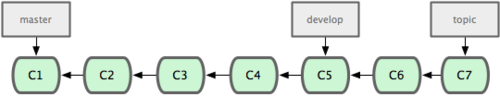
\includegraphics[width=0.5\textwidth]{img/longterm.png}
	\caption{Langfristige Brances}
\end{figure}
\subsection{Themen Branches}
Kurzlebige Zweige für die Entwicklung spezieller Features und Funktionen. Diese Branches liegen nur lokal vor.
\begin{figure}[ht]
	\centering
		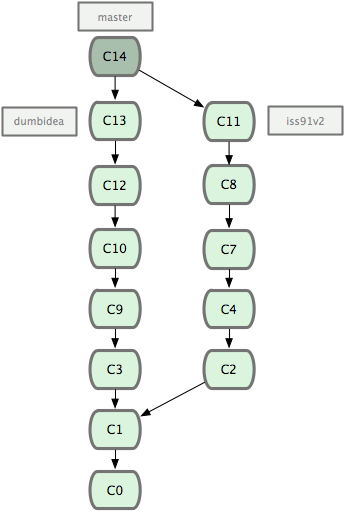
\includegraphics[width=0.22\textwidth, angle=90]{img/thema.png}
	\caption{Themen Branches}
\end{figure}
\section{Externe Branches}
\section{Rebasing}
In Git gibt es zwei Methoden Änderungen in einen anderen Branch zu überführen. Neben dem \texttt{merge} existiert das \texttt{rebase} Kommando.
\subsection{einfaches Rebase}
Bei einem einfachen Rebase wird der Vorfahr eines Zweiges geändert. Dies dient dazu einen 3-Wege-Merge zu vermeiden, sodass ein einfacher Fast-Forward-Merge durchgeführt werden kann.
\begin{lstlisting}[caption={Einfaches Rebase},captionpos=b]
#Branch to rebase
git checkout dev

#Rebase Branch
git rebase master

#Change to Master and merge
git checkout master
git merge dev

#Rebase without Checkout
rebase [Basis-Branch] [Themen-Branch]
\end{lstlisting}
\subsection{Rebasing auf anderen Branch}
\begin{lstlisting}[caption={Rebase auf anderen Branch},captionpos=b]
git rebase --onto master server client
\end{lstlisting}
\begin{figure}[ht]
	\centering
		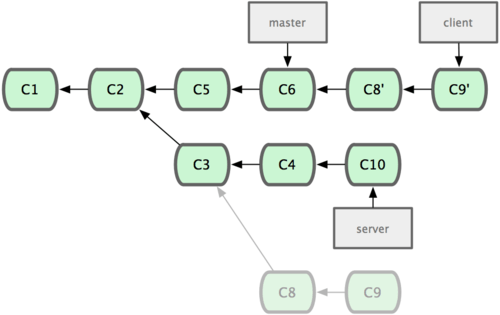
\includegraphics[width=0.6\textwidth]{img/rebase.png}
	\caption{Themen Branches}
\end{figure}
\textbf{Rebase keine Commits die in ein öffentliches Repository hochgeladen wurden}


\chapter{Server}
\section{Protokolle}
\subsection{Lokales Protokoll}
\subsection{SSH Protokoll}
\subsection{Git Protokoll}
\subsection{HTTP/S Protokoll}




%\input{}

\chapter{Changelog}
\large\textbf{V1.0 - 2017.08.20}\\[-1.5em]
\begin{itemize}
\item Erstveröffentlichung
\end{itemize}

\end{document}
